%% ----------------------------------------------------------------
%% Chapter 2: Theoretical background
%% ----------------------------------------------------------------
%!TeX root = subfile
\label{chapter:theoretical_background}
\documentclass[../main.tex]{subfiles}
% ----------------------------------------------------------------
\begin{document}

\vspace{0.25cm}
This chapter comprises high-level theoretical background in incompressible fluid flow and its numerical solution.
The incompressible flow dynamics is first presented yielding the governing system of equations.
The numerical method providing an approximate solution of the equation system is also explained as implemented in our in-house code, ``Lotus''.
A finite-volume method is employed to spatially discretise the system domain.
The flux-limited quadratic upstream interpolation for convective kinematics (QUICK) scheme numerically approximates the convective term of the momentum equations, which also serves as an implicit model for the subgrid scale (SGS) structures of the flow.
A central-difference scheme is used for the viscous term.
A predictor-corrector scheme integrates the numerical solution in time.
The boundary data immersion method is applied to account for solid boundaries.
Finally, a multigrid method is employed to iteratively solve the pressure-Poisson equation and enforce the continuity condition in the velocity field.

\section{Governing equations of incompressible fluid flow}

Incompressible fluid flow is governed by the conservation of mass and momentum, respectively the continuity equation and the Navier--Stokes momentum equations
\begin{gather}
\nabla\cdot\vect{u}=0,\label{eq:div_u}\\
\pd{\vect{u}}{t}+\pars{\vect{u}\cdot\nabla}\vect{u}=-\nabla p+\nu\nabla^2\vect{u},\label{eq:n-s}
\end{gather}
where $\vect{u}\left(\vect{x}, t\right) = \left(u, v, w\right)$ is the velocity vector field, $p\left(\vect{x}, t\right)$ is the pressure field, $t$ is the time, and $\vect{x}=\left(x,y,z\right)$ is the spatial vector.
The coupling of pressure and velocity arises from an additional relationship obtained by taking the divergence of the momentum equations, namely the pressure-Poisson equation
\begin{gather}
\nabla\cdot\pars{\pd{\vect{u}}{t}+\pars{\vect{u}\cdot\nabla}\vect{u}=-\nabla p+\nu\nabla^2\vect{u}},\\
\nabla^2 p = \nabla\cdot\pars{\vect{h}-\pd{\vect{u}}{t}},\label{eq:ppe}
\end{gather}
where $\vect{h}$ is the force combining convective and viscous terms.

The system of equations is bounded by case-dependant initial and boundary conditions of the system variables.
Importantly, the boundary condition with solid domains is the velocity no-slip condition, i.e. $\vect{u}_b=0$, which yields the flow boundary layer.

The Reynolds number is the non-dimensional parameter describing the ratio between convective and viscous forces,
\begin{equation}
Re=\frac{\rho U L}{\mu},
\end{equation}
where $\rho$ is the fluid density (assumed constant for incompressible flows), $\mu$ is the dynamic fluid viscosity, and $L$ and $U$ are the characteristic length and velocity of the system, respectively.
The Reynolds number defines the scales of motion of the flow.
When the convective forces are much greater than the viscous forces, turbulence develops.
The definition of turbulence is not straight forward, but (loosely) it can be thought as the turning point where the fluid dynamics transitions from ordered to \textit{chaotic} as a result of the nonlinear convective term.
Still, physical laws revealing certain order within the turbulence dynamics have been found in the past.
In particular, it is known that 3-D systems present a constant rate of kinetic energy transfer within a certain range of scales, from large to small structures, a.k.a. direct energy cascade \citep{Richardson1922,Kolmogorov1941}.
Similarly, a constant rate is also found in 2-D systems although energy is inversely transfered from small to large scales, a.k.a. inverse energy cascade \citep{Kraichnan1967,Leith1968,Batchelor1969}.
Such different dynamics will be subject of investigation in the following chapters.

\section{Numerical methods}
\label{sec:lotus}

\subsection{Spatial discretisation}

The governing equations comprising \eref{eq:div_u}, \eref{eq:n-s}, and \eref{eq:ppe} are spatially discretised in a structured rectilinear grid using a finite-volume method.
This grid facilitates the implementation of the immersed boundary method accounting for solid boundary conditions, as described in \sref{sec:bdim}.
The flow variables, pressure and velocity, are staggered: the pressure scalar field is stored in the cell centre and the velocity vector field is defined at the cell faces, as displayed in \fref{fig:grid}.

\begin{figure}[t]
\centering
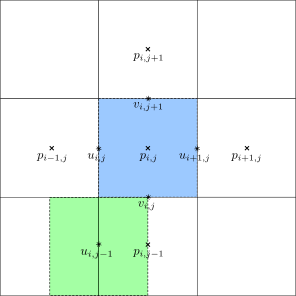
\includegraphics[width=0.4\linewidth]{chapter2/staggered_grid}
\caption{Staggered grid.
The control volume for the pressure is defined in blue.
The control volume for the $u$ velocity component is defined in green.}
\label{fig:grid}
\end{figure}

The convective term of the momentum equations is numerically approximated using a flux-limited QUICK scheme.
This scheme interpolates the quantity of interest at the control volume face through a weighted quadratic function fitted with one upstream and two downstream points \citep{Leonard1979}.
The spatial derivative is then approximated using the numerical fluxes given by the cell-face values as defined by the finite-volume approach.

\subsection{Implicit modelling}

As previously exposed, high-Reynolds flows need to be sufficiently discretised in space and time to fully resolve all scales of motion.
The spatial SGS need to be modelled when the grid is not fine enough.
In this sense, we employ an implicit LES (iLES) model, in which the dissipative effect of the SGS is accounted by the numerical dissipation intrinsic in the discretisation scheme of the convective term (the QUICK scheme in the present solver).

Importantly, the instantaneous kinetic energy $(E)$ dissipation rate $(\epsilon)$
\begin{equation}
\dd{E}{t}=-\epsilon
\end{equation}
needs to match the natural dissipation mechanism of the flow.
This balance can be used to compute the iLES effective Reynolds number (or effective kinematic viscosity, $\nu_e$), which can be found through the following evaluation \citep{Domaradzki2003,Aspden2008,Zhou2014}
\begin{equation}
\dd{}{t}\int_\Omega\frac{1}{2}|\vect{u}|^2\,\mathrm{d}\Omega=-2\nu\int_\Omega S_{ij}S_{ij}\,\mathrm{d}\Omega,\label{eq:iles}
\end{equation}
where $S_{ij}$ is the velocity rate-of-strain tensor.
Note that the RHS is the energy dissipation term for incompressible flow arising naturally in the energy transport equation (formally derived from a dot product of the Navier--Stokes momentum equations and the velocity vector field) since \citep[p. 17]{Doering1995}
\begin{equation}
\frac{1}{2}\int_\Omega||\nabla\vect{u}||^2\,\mathrm{d}\Omega=\frac{1}{2}\int_\Omega|\boldsymbol{\omega}|^2\,\mathrm{d}\Omega\equiv Z,
\end{equation}
where $\boldsymbol\omega=\nabla\times\vect{u}$ is the vorticity vector field, $Z$ is the enstrophy, and $||\cdot||$ denotes the tensor Frobenius norm.

Using \eref{eq:iles}, the iLES effective viscosity is computed as
\begin{equation}
\nu_e=\frac{\avg{\epsilon}_{\scaleto{\Omega}{5pt}}}{2\avg{S_{ij}S_{ij}}_{\scaleto{\Omega}{5pt}}},
\end{equation}
where $\avg{\cdot}_{\scaleto{\Omega}{5pt}}$ denotes a volume average.
\cite{Hendrickson2019} verified the present in-house solver by monitoring the grid-scaled effective viscosity $\nu_e\Delta^{-1}$ for the Taylor--Green vortex case.
It was shown that the QUICK scheme linearly scales the effective viscosity with $\Delta$.

\subsection{Temporal discretisation}

The temporal evolution of the system of equations (\eref{eq:div_u}, \eref{eq:n-s} and \eref{eq:ppe}) is discretised using Chorin's projection method \citep{Chorin1967,Chorin1968}.
In short, the Navier--Stokes operator is split in two parts
\begin{gather}
\frac{\vect{u}^*-\vect{u}^n}{\delta t}=\nu\nabla^2\vect{u}^n-\pars{\vect{u}^n\cdot\nabla}\vect{u}^n,\\
\frac{\vect{u}^{n+1}-\vect{u}^*}{\delta t}=-\nabla p^{n+1},
\end{gather}
where the superscript $(\cdot)^n$ refers to the time step level and the intermediate velocity field is noted with the superscript $(\cdot)^*$.
The computation of a non-solenoidal intermediate velocity field allows to decouple the velocity and pressure equations.
In this way, a solenoidal velocity field $\vect{u}^{n+1}$ can be obtained by enforcing the continuity condition into the $p^{n+1}$ pressure-Poisson equation.
Otherwise, using $p^{n}$ to compute $\vect{u}^{n+1}$ would not enforce the velocity field to be divergence-free at the next time step.

The projection method is implemented in a predictor-corrector algorithm.
Next, we note $\vect{h}(\vect{u})=\nu\nabla^2\vect{u}-\pars{\vect{u}\cdot\nabla}\vect{u}$, and $\vect{h}^n=\vect{h}(\vect{u}^n$).
The $(\cdot)^s$ superscript refers to a solenoidal field.
With this, the predictor-corrector algorithm is implemented in two steps as follows

\begin{align}
\mathrm{Pred}&\mathrm{ictor\,\,step:}\nonumber\\
&1.\qquad \vect{u}^* = \vect{u}^n+\vect{h}^n\delta t,\\
&2.\qquad {\delta t}\,\nabla^2p^*=\nabla\cdot\vect{u}^*,\label{eq:ppe1}\\
&3.\qquad \vect{u}^{*,s}=\vect{u}^*-\delta t\nabla p^*.
\nonumber\\
\nonumber\\
\mathrm{Corr}&\mathrm{ector\,\,step:}\nonumber\\
&4.\qquad \vect{u}^{*} = \vect{u}^n+\frac{1}{2}\pars{\vect{h}^n+\vect{h}^{*,s}}\delta t,\\
&5.\qquad {\delta t}\,\nabla^2p^{n+1}=\nabla\cdot\vect{u}^{*},\label{eq:ppe2}\\
&6.\qquad \vect{u}^{n+1}=\vect{u}^{*}-\delta t\nabla p^{n+1}.
\end{align}

Note that the divergence-free constraint for both $\vect{u}^n$ and $\vect{u}^{n+1}$ has been considered.
Also note that the forward Euler time stepping scheme is implemented in the predictor step to compute the intermediate velocity field $\vect{u}^{*}$, finally projected into a solenoidal field by the pressure-Poisson equation yielding $\vect{u}^{*,s}$.
With this, the trapezoidal quadrature can be employed in the corrector step to integrate the solution from time $n$ to $n+1$, as described in step 4.
The solution is again projected into a divergence-free field by solving the pressure-Poisson equation for $p^{n+1}$ (step 5) and correcting the velocity field with the new pressure field (step 6) yielding $\vect{u}^{n+1}$.

The advantage of this method is that it exploits the benefits of both explicit and implicit time-marching schemes: it combines the natural stability of implicit schemes with the low memory requirements of explicit schemes.
It can be shown that the predictor-corrector algorithm is second-order accurate in time.
The reader is referred to \cite{Ferziger2002} for further details.

The time discretisation method is bounded to the limitation of the time step size $(\delta t)$.
For this, the local Courant number $(u\,\delta t/\delta x)$ and Péclet number $(\nu\,\delta t/(\delta x)^2)$ are evaluated at every time step yielding an adaptive step size.
These dimensionless parameters quantify the characteristic convection time and characteristic diffusivity time of the flow, respectively.
A combination of both yields to a time step size limit (for  one-dimensional flow) of
\begin{equation}
\delta t<\left[\frac{2\nu}{\min\left[(\delta x)^2\right]}+\max\pars{\frac{u}{\delta x}}\right]^{-1}.
\end{equation}


\subsection{Solid boundaries} \label{sec:bdim}

The velocity no-slip condition at solid boundaries is implemented using the boundary data immersion method (BDIM) from \cite{Weymouth2011}.
Immersed boundary (IB) methods, such as BDIM, take into account the solid wall effect in a rectilinear non-conforming grid.
The Dirichlet condition on the velocity field is interpolated at the grid nodes from its actual position.
The interpolation method is what differs among IB methods.

A clear advantage of IB methods is the trivial grid-generation process, in contrast to the complicated meshing process regularly encountered for body-conforming grids.
Also in this regard, the body geometry is practically irrelevant for the grid generation process.
Other advantages include the simulation of moving bodies since the grid does not need to be updated at every step, as well as the straightforward implementation of numerical schemes.
On the other hand, accuracy near the solid boundary can be compromised depending on the effective resolution of the non-conforming grid.
Also, the implementation of the solid boundary condition is not as trivial as in body-conforming grids \citep{Mittal2005}.

The BDIM consists in mapping the fluid governing equation $(\mathcal{F})$ and the solid governing equation $(\mathcal{B})$ into a single meta-equation $(\mathcal{M})$ discretised in a non-conforming rectilinear staggered grid.
A convolution kernel $(K_\epsilon)$ provides a smooth transition between the mediums enforcing the velocity condition at the interface (see \fref{fig:bdim}) while extending the fluid subdomain $(\Omega_f)$ and solid subdomain $(\Omega_b)$ to the full single domain $(\Omega)$.
Imposing the no-slip condition on a static body, this method can be summarised as follows
\begin{align}
&\mathcal{F}(\vect{u},p)=\partial_t\vect{u}-\vect{h}+\nabla p=0,\\
&\mathcal{B}(\vect{u})=\vect{u}=0,\\
&\mathcal{M}(\vect{u},p)=\mathcal{F}(\vect{u},p)\pars{1-\delta_\epsilon}+\mathcal{B}\pars{\vect{u}}\delta_\epsilon=0,
\end{align}
where the convolution between kernel and governing equation has been approximated using (e.g)
\begin{gather}
\mathcal{B}_\epsilon\pars{\vect{x}}=\int_{\Omega_b}\mathcal{B}\pars{\vect{x}_b}K_\epsilon\pars{\vect{x},\vect{x}_b}\,\mathrm{d}\vect{x}_b\approx \mathcal{B}\pars{\vect{x}}\int_{\Omega_b}K_\epsilon\pars{\vect{x},\vect{x}_b}\,\mathrm{d}\vect{x}_b,\\
\mathcal{B}_\epsilon\pars{\vect{x}}\approx\mathcal{B}\pars{\vect{x}}\delta_\epsilon,
\end{gather}
where $\delta_\epsilon$ is the integrated kernel over the subdomain which can take the approximated form
\begin{equation}
\delta_\epsilon(d)=
	\begin{cases}
		\frac{1}{2}[1+\sin(\frac{\pi}{2}\frac{d}{\epsilon})] & \mathrm{for} \left|d\right|<\epsilon\\
		1 & \mathrm{for}\,\,d<-\epsilon\\
		0 & \mathrm{else}
	\end{cases}
\end{equation}
where $d$ is a signed-distance function from a point $\vect{x}$ to the solid interface. This approximation results into a first-order accurate scheme, although high-order terms can be considered to improve the order of accuracy \citep{Maertens2015}.

The BDIM has been tested in multiple applications and the reader is referred to \cite{Maertens2015} for an extended mathematical description of the method, and to \cite{Schulmeister2017} for further validation on bluff body cases.

\begin{figure}[t]
\centering
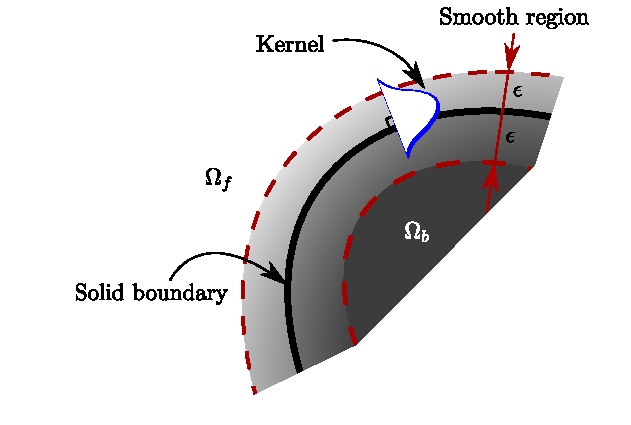
\includegraphics[width=0.65\linewidth]{chapter2/bdim}
\caption{BDIM sketch adapted from \cite{Maertens2015}.
A convolution kernel with radius $\epsilon$ smooths the interface between solid $(\Omega_b)$ and fluid $(\Omega_f)$ subdomains.}
\label{fig:bdim}
\end{figure}

\subsection{Pressure solver}

A multigrid method is used to solve the pressure-Poisson equation as discretised in the pressure-corrector algorithm (\eref{eq:ppe1} and \eref{eq:ppe2}).
Algebraically, the pressure-Poisson equation can be written as a linear system of equations
\begin{equation}
\matr{A}\vect{x}=\vect{b},
\end{equation}
where $\matr{A}$ is a sparse matrix containing the discretised Laplacian operator, $\vect{x}$ is the pressure field arranged in a column vector, and $\vect{b}$ is the column vector of the intermediate velocity field divergence.

Contrary to direct methods, a multigrid solver is an iterative method in the sense that that a guessed solution $\vect{x}^n$ (at the iteration $n$) is evaluated yielding a residual
\begin{equation}
\vect{r}^n=\matr{A}\vect{x}^n-\vect{b},
\end{equation}
and an error
\begin{equation}
\boldsymbol\epsilon^n=\vect{x}-\vect{x}^n,
\end{equation}
which are related by
\begin{equation}
\matr{A}\boldsymbol\epsilon^n=\vect{r}^n.
\end{equation}
The objective is to iteratively minimise $\vect{r}^n$ so that $\vect{x}^n$ converges to $\vect{x}$.

In multigrid methods, iterations are performed from fine to coarse grids, transferring the residual across grid levels so that iterations become cheaper as the grid is coarsened.
Hence, multigrid methods yield a speed-up of the overall convergence process.
Iterations can be carried with any iterative method, e.g. Gauss--Seidel, Jacobi, conjugate gradient, etc.
In our solver, a single Jacobi iteration to smooth the solution is performed before downsampling the residual to a coarser level.
Downsampling (in one-dimensional form) is performed from
\begin{equation}
\frac{1}{(\delta x)^2}\pars{\epsilon_{i-1}^n-2\epsilon_{i}^n+\epsilon_{i+1}^n}=r_i^n,
\end{equation}
where the subscript $(\cdot)_i$ denotes the fine grid cell index, to
\begin{equation}
\frac{1}{(\delta X)^2}\pars{\epsilon_{I-1}^n-2\epsilon_{I}^n+\epsilon_{I+1}^n}=r_I^n,
\end{equation}
where the subscript $(\cdot)_I$ denotes the coarse grid cell index.
The relationship between both grids might be $\delta X = 2\delta x$, hence the $I$ (coarse grid) control volume is defined as the $i$ (fine grid) control volume plus half of its neighbour control volumes ($i+1$ and $i-1$) \citep{Ferziger2002}.

The residual can be gradually downsampled to an arbitrary coarse grid using linear interpolation for each downsampling step.
Similarly, the residual is upsampled from the coarsest grid to the original fine grid while iterating in the mid level grids to correct the fine grid solution.
We employ a conjugate gradient method after each upsampling step to update the solution.
This downsampling and upsampling process is known as a V-cycle.
Multiple V-cycles can be performed in a single time step to solve the pressure-Poisson equation.
The iterative method is stopped once the convergence tolerance is reached.
The following convergence tolerance criteria is defined in a grid with cell index $i$
\begin{gather}
\frac{1}{\Omega}\sum_i\Big|\oint \vect{u}\cdot\vect{\hat{n}}\,\mathrm{d}S\Big|<10^{-6}\\
\max_i\Big|\oint \vect{u}\cdot\vect{\hat{n}}\,\mathrm{d}S\Big|<10^{-5} \,\,\, \forall i \in \Omega ,
\end{gather}
establishing the allowed average velocity divergence error in $\Omega$ as well as its maximum local error.
% ---------------------------------------------------------------- 
\end{document}